\documentclass[ngerman]{scrartcl}
\usepackage[utf8]{inputenc}
\usepackage[T1]{fontenc}
\usepackage{babel}
\usepackage{csquotes}
\usepackage{lmodern}
\usepackage{microtype}

\usepackage{amsmath, amssymb}
\usepackage{scrlayer-scrpage}
\usepackage{graphicx}
\usepackage{xcolor}
\usepackage{booktabs}
\usepackage{tabularx}
\usepackage{placeins}
\usepackage[sorting=nyt, backend=biber, citestyle=numeric]{biblatex}
\bibliography{Bibliography}
\usepackage[output-decimal-marker={,}]{siunitx}

\usepackage{hyperref}
\hypersetup{
	colorlinks,
	citecolor=blue,
	filecolor=blue,
	linkcolor=black,
	urlcolor=blue
}
\usepackage[figure, table]{hypcap}
\usepackage{xcolor}

\newcommand{\abs}[1]{\ensuremath{\left\vert#1\right\vert}}


\title{Theoretische Physik IV}
\subtitle{Thermodynamik und Quantenstatistik}
\author{Prof. Dr. Tilo Wettig}
\date{21.05.2017}



\begin{document}
	
	
	\maketitle
	\thispagestyle{empty}
	\vspace{2cm}
	\begin{minipage}{\linewidth}	
		\centering
		\includegraphics[width=0.4\linewidth]{LOGO_UR.eps}	
	\end{minipage}
		
	\newpage
	\tableofcontents
	\newpage
	
	\section{Einführung}
	
		\begin{itemize}
			\item \textbf{Statistische Physik:}\begin{itemize}
					\item Wir betrachten Systeme mit sehr viele Teilchen ( z.B. Gas, 									Flüssigkeit mit $\mathcal{O}(10^4)$ Teilchen)
					\item Dynamik der Teilchen durch Mechanik/Quantenmechanik bestimmt, aber Gesamtheit der Bewegungsgleichungen nicht lösbar
					\item stattdessen: statistische Behandlung, d.h. Betrachtung von Wahrscheinlichkeiten für Zustände des Systems
					
			\end{itemize}
				\item \textbf{Thermodynamik:}\begin{itemize}
						\item Aussagen über makroskopische Größen, z.B. Temperatur oder Druck, bzw. deren Beziehungen untereinander 
						\item kann aus der statistischen Physik hergeleitet werden, aber historisch wurde die Thermodynamik ohne Bezug auf mikroskopische Grundlagen hergeleitet
			\end{itemize}
			\item betrachte ein statistisches Experiment mit\begin{itemize}
					\item $N$ = Zahl der Versuche
					\item $i$ = Index für mögliche Ergebnisse/Ereignisse
					\item $N_i$ = Anzahl des Auftretens ders Ergebnisses $i$
					\item \textbf{Zeitmittel}\dotso führe das gleiche Experiment N mal hintereinander durch
					\item \textbf{Ensemblemittel}\dotso führe N gleichartige Experimente je einmal durch
					\item im Einzelfall muss immer geklärt werden, unter welchen Bedingungen Zeitmittel und Ensemblemittel übereinstimmen 
			\end{itemize}
			\item \textbf{Beispiel 1:} Würfel\begin{itemize}
						\item Zeitmittel: würfle N mal mit demselben Würfel
						\item Ensemblemittel: würfle je einmal mit N Würfeln
						\item Zeit- und Ensemblemittel sind gleich, wenn für alle Würfel die Zahlen eins bis sechs gleich wahrscheinlich sind ($p_i = \frac{1}{6}$)
			\end{itemize}
			\item \textbf{Beispiel 2:} Bestimmung der kinetischen Energie $\varepsilon_i$ der Atome in einem Gas\begin{itemize}
						\item die Energie ändert sich ständig durch Stöße der Atome untereinander, mit mittlerer Stoßzeit $\tau \approx 10^{-10}~s$
						\item Zeitmittel: betrachte ein Atom und messe dessen Energie N mal
						\item Ensemblemittel: messe einmalig die Energie von N Atomen
						\item Zeitmittel=Ensemblemittel, wenn beim Zeitmittel gilt: \newline Abstand der Messungen $\gg\tau$ 
			\end{itemize}
			\item betrachte nun N gleichartige Systeme die in diskreten Zuständen $i$ vorliegen\begin{itemize}
					\item in Beispiel 1: System=würfel, Zustände= 1\dots 6
					\item in Beispiel 2: System=Atom, Zustände=Energieintervalle um $z_i$
					\item falls sich zwei Zustände ausschließen, gilt: \[
					p_{i oder j}=p_i + p_j
					\]
			\end{itemize}
			\item Mittelwert und Schwankung:\begin{itemize}
					\item betrachte eine Größe x, die im Zustand i den Wert $x_i$ hat (Würfel: $x_i=i$, Atom: $x_i=\varepsilon_i$)
					\item Mittelwert: \[ \bar{x} = \sum_i p_i x_i\]
					\item die $x_i$ weichen vom Mittelwert ab, mit mittlerer Abweichung:
						\[ \overline{x - \bar{x}} = \sum_i p_i (x_i - \bar{x})= \sum_ip_ix_i - \bar{x}\sum_i p_i = \bar{x} - \bar{x} = 0 \]
					\item daher definiert man als Maß für die Abweichung von Mittelwert die mittlere quadratische Abweichung oder Schwankung \[ \Delta x = \sqrt{\overline{x - \bar{x}}}
\]					
							es gilt:
							\begin{gather}
								(\Delta x)^2=\sqrt{\overline{(x-\bar{x})^2}}=
								\sum_i p_i(x_i - \bar{x})^2 = 
								\sum_i p_i x_i^2 -2\bar{x}\sum_i p_i x_i + \bar{x}^2\sum_ip_i \\= \overline{x^2} - 2\bar{x}^2 +\bar{x}^2=\overline{x^2} - \bar{x}
							\end{gather}
			\end{itemize}
			
			\item \textbf{Schlussbewertung:} strenggenommen muss man unterscheiden zwischen Mittelwert ( normalerweise definiert für endliche N ) und Erwartungswert ( eines Mittelwerts für $N \rightarrow \infty$)
			
			
		\end{itemize}
		
	\section{Mathematische Grundlagen}
	
	\subsection{Binomialverteilung und Gesetz der großen Zahl}\label{sec:binom}
	
	
	Betrachte nun einen \enquote{random walk} in einer Dimension (x-Achse) mit folgenden Regeln:
	\begin{itemize}
		\item starte bei $x=0$
		\item springe mit Wahrscheinlichkeit p (bzw. q) um $\Delta x =1$ (bzw. $\Delta x = -1$)
		\item es gilt $p+q=1$
	\end{itemize}
	
	
	Die Anzahl der positiven (bzw. negativen) Schritte sei $n_+$ (bzw.. $n_-$) und die Gesamtzahl sei $N=n_+ + n_-$. Im Folgenden berechnin wir
	\begin{itemize}
		\item $P_N(m)$ \ldots Wahrscheinlichkeit, bei $x=m=n_+ - n_-$ anzukommen
		\item $W_N(n)$ \ldots Wahrscheinlichkeit, dass $n = n_+$ positive Schritte durchgeführt werden
		\item Mittelwerte $\bar{m}$ und $\bar{n}$
		\item Schwankungen $\Delta m$ und $\Delta n$
		
	\end{itemize}
	
	Betrachte zunächst als Beispiel $N=5$. 
	\begin{itemize}
		\item der random walk (1, -1, -1, 1, 1) hat die Wahrscheinlichkeit $pqqpp=p^3q^2$ und ergibt $m=1$ und $n=3$
		\item es gibt noch andere Möglichkeiten, bei $m=1$ anzukommen, z.B. (-1, -1, 1, 1, 1); diese haben auch Wahrscheinlichkeit $p^3q^2$
		\item da sich diese Möglichkeiten ausschließen, müssen wir über sie summieren
		\item Anzahl der Möglichkeiten ist $\binom{5}{3}$ und damit \[ P_5(1)=W_5(3)=\frac{5!}{3! \cdot 2!}p^3q^2 \]
	\end{itemize}
	
	Nun betrachten wir den allgemeinen Fall. Jeder Weg mit $n_+$ positiven und $n_-$ negativen Schritten hat die Wahrscheinlichkeit $p^{n_+}q^{n_-}$ und die Anzahl der verschiedenen Wege ist $\binom{N}{n_+} = \binom{N}{n}$, woraus folgt:
	\begin{equation}
		P_N(m)=W_N(n)=\binom{N}{n}p^n q^{N-n} \tag{Binomialverteilung}
	\end{equation}
	
	Überprüfe, dass die Summe aller Wahrscheinlichkeiten 1 ist:
	\begin{equation}
		\sum_{n=0}^N W_N(n) = \sum_{n=0}^N n \binom{N}{n}p^n q^{N-n} = 1 ~~\checkmark
	\end{equation}
	
	Berechne Mittelwert:
	\begin{gather}
		\sum^N_{n=0} W_N(n)n = 
		\sum_{n=0}^N n\binom{N}{n} p^n  q^{N-n} = 
		\\p\sum_{n=0}^{N}\binom{N}{n} p^n q^{N-n}=
		p\frac{\partial}{\partial p} (p+q)^N = pN(p+q)^{N-1}=pN
	\end{gather}
	Analog gilt:
	\begin{equation}
		\overline{n_-} = qN \hspace{2cm} \overline{m} = \langle n_+\rangle - \langle n_-\rangle = (p-q)N
	\end{equation}
	
	Berechne Schwankungen:
	
	\begin{gather}
		\langle n^2 \rangle = \sum_{n=0}^N n^2 ~\binom {N}{n}~ p^n q^{N-n} = p \frac{\partial}{\partial p}~ p \frac{\partial}{\partial p} ~\sum_{n=0}^N \binom{N}{n}~ p^n q^{N-n}=\\
		p \frac{\partial}{\partial p}~ p \frac{\partial}{\partial p}~(p+q)^N = p \frac{\partial}{\partial p}~ pN(p+q)^{N-1} = pN + p^2N(N-1) \\= p(1-p)N + (pN)^2 = pqN + \bar{n}^2
	\end{gather}
	
	Ein Beispiel für einen random walk wären N Gasatome im Volumen V. Teile V in zwei Teilvolumina ein(siehe \autoref{fig:random_walk}). Jedes Atom list mit gleicher Wahrscheinlichkeit am gleichen Ort. Also ist ein Atom mit Wahrscheinlichkeit p (bzw. q) im linken (bzw rechten) Teil. Dann ist $W_N(n)$ die Wahrscheinlichkeit, dass genau n Atome im linken Teil sind. Im Mittel sind $\bar{n}=pN$ Atome im links. Wegen der Bewegung der Gasatome fluktuiert die anzahl der Atome im linken Teil um $\bar{n}$ , mit Schwankung $\Delta n$. Für $p=q=\frac{1}{2}$ gilt:
	
	\begin{equation}
		\bar{n}=0,5 \cdot 10^{24} \hspace{1.5cm} \Delta n = \sqrt{\frac{1}{4}10^{24}}=0,5\cdot 10^{12} \hspace{1.5cm}  \frac{\Delta n}{n}=10^{-12}
	\end{equation}
	
	\begin{figure}[h]
		\centering
		\includegraphics[width=0.7\linewidth]{random_walk}
		\label{fig:random_walk}
		\caption{Schematische Darstellung des Volumens beim random walk}
	\end{figure}
	
	
	\subsection{Normalverteilung}
	
	Für große N hat $W_N(n)$ ein scharfes Maximum bei $n=\bar{n}$, also entwickeln wir $W_N(n)$ um diesen Punkt. Wegen des Auftretens von Faktoren wie $p^n$ entwickeln wir den Logarithmus:
	\begin{equation}
		ln W_N(n)=ln~N! - ln~n ! - ln(N-n)!
	\end{equation} %%%%%%%% hier fehlt mir ne Formel, zu langsam ;D
	
	Für $n\gg 1$ gilt:
	
	\begin{equation}
		\frac{d}{dn}\approx\frac{ln(n+1)! - ln~n!}{1}=ln(n+1)\approx ln~n
	\end{equation}
	und damit:
	\begin{equation}
		\frac{d}{dn}ln~W=-ln~n + ln(N-n) + ln~p - ln~q \underbrace{=}_{n=\bar{n}} = 0
	\end{equation}
	
	Dies gilt für $\bar{n}\gg 1$ und $N-\bar{n}\gg 1$, also für $pqN\gg 1$. $W_N(n)$ hat also bei $n=\bar{n}$ ein Extremum. Berechne zweite und dritte Ableitung (für später):
	
	\begin{equation}
		\frac{d}{dn}ln~W = -\frac{1}{n} - \frac{1}{N-n} = - \frac{1}{pqN}=-\frac{1}{(\Delta n)^2} < 0
	\end{equation}
	
	\begin{equation}
		\frac{d}{dn^2}ln~W = \frac{1}{n^2} - \frac{1}{(N-n)^2} = \frac{q^2-p^2}{(\Delta n)^4}
	\end{equation}
	
	Damit ergibt sich
	\begin{equation}
		ln~W_N(n)=ln~W_N(\bar{n}) - \frac{(n-\bar{n})^2}{2(\Delta n)^4} + \mathcal{O}\left((n-\bar{n})^3\right)
	\end{equation}
	
	Nun berechnen wir $W_N(\bar{n})$ über die Normierung der Wahrscheinlichkeit:
	
	\begin{gather}
		1 = \sum_{n=0}^N W_N(n) \approx \int_0^N W_N(x)dx \approx \int_{-\infty}^{\infty} W_N(x)dx =\\ 
		W_N(\bar{n}) \int_{-\infty}^{\infty} \exp\left(-\frac{(x-\bar{n})^2}{2(\Delta n)^2}\right)dx= W_N(\bar{n}) \sqrt{2\pi} \Delta n
	\end{gather}
	
	und damit:
	
	\begin{equation}
		W_N(n)=\frac{1}{\sqrt{2\pi}\Delta n}\exp\left( -\frac{(n-\bar{n})^2}{2(\Delta n)^2}\right)
	\end{equation}
	
	Für die Verallgemeinerung des random walk auf beliebige Schrittlänge l ist:
	\begin{equation}
		x=nl \hspace{2cm} \bar{x}=\bar{n}l \hspace{2cm} \sigma :=\Delta x= \Delta nl
	\end{equation}
	
	Wir definieren zusätzlich die Wahrscheinlichkeitsdichte $P(x)$:
	\begin{equation}
		P(x)dx=\begin{cases}~&\textit{Wahrscheinlichkeit, die Zufallsgröße x} \\~&\textit{im Intervall (x, x+dx) zu finden}\end{cases}
	\end{equation}
	
	Für ein Intervall mit $\frac{dx}{l}\gg 1 $ gilt:
	\begin{equation}
		P(x)dx=\sum_{n' in dx} W_N(n') \approx \int_{\frac{x}{l}}^{\frac{x+dx}{l}} dn'~W_N(n')\approx\frac{dx}{l}~W_N(n)
	\end{equation}
	
	Damit folgt:
	
	\begin{equation}\tag{Normalverteilung}
		P(x)=\frac{1}{\sqrt{2\pi}\sigma}\exp\left(-\frac{(x-\bar{x})^2}{2\sigma}\right)
	\end{equation}
	
	Diese Verteilung gilt auch für stetige Zufallsgrößen x. $\sigma =\Delta x$ heißt Standardabweichung. 
	
	\begin{figure}[h]
		\centering
		\includegraphics[width=0.85\linewidth]{Normalverteilung.png}
		\label{fig:normalverteilung}
		\caption{Graph der Normalverteilung P(x)}
	\end{figure}
	
	Es gilt:
	\begin{equation}
		\int_{x1}^{x_2} P(x)dx= \textit{Wahrscheinlichkeit, x im Intervall} ~(x_1, x_2)~ \textit{zu finden}
	\end{equation}
	\begin{equation}
		\int_{-\infty}^{\infty} P(x)dx = 1
	\end{equation}
	
	\begin{equation}
		\int_{\bar{x} - k\sigma}^{\bar{x} + d\sigma} P(x)dx =
		\begin{cases}
			0,683 & k=1\\
			0,954 & k=2\\
			0,997 & k=3\\
		\end{cases}
	\end{equation}
	
	Folglich sind Ereignisse außerhalb eines $\sigma$ -Intervalls $32~\%$ wahrscheinlich, aber außerhalb nur noch $0,3~\%$ wahrscheinlich. Damit die Normalverteilung gilt, muss in Taylerentwicklung gelten: 3.Ordnung $\ll$ 2.Ordnung:
	\begin{equation}
		\abs{\frac{ln~W'''~(n-\bar{n})^3}{ln~W''~(n-\bar{n})^2}} \leq \frac{|n-\bar{n}|}{(\Delta n)^2}
	\end{equation}
	
	Wegen $n-\bar{n}\approx k\Delta n $ mit $k=\mathcal{O}(1)$ bedeutet dies $\Delta n \gg 1$ bzw. $pqN\gg 1$. Für sehr kleines p (oder q) ergibt sich statt der Normalverteilung eine Poissonverteilung.
	
	\subsection{Zentraler Grenzwertsatz}
	
	\noindent\hspace{0.15\linewidth}\begin{minipage}{0.77\linewidth}
	\vspace{1cm}
	 Wenn die Größe $x=\sum_{i=0}^N s_i$ die Summe vieler Zufallszahlen $s_i$ ist, dann ist die Wahrscheinlichkeitsdiche $P(x)$ eine Normalverteilung (unabhängig davon, wie die $s_i$ verteilt sind).
	 
	 \vspace{0.2cm}\textit{- Zentraler Grenzwertsatz}
	\end{minipage}\vspace{1cm}
	
	Die Wahrscheinlichkeitsdichte von $s_i$ sei $w_i(s_i)$ und alle Momente der $s_i$ seien endlich mit:
	\begin{equation}
			\int_{-\infty}^{\infty} w_i(s_i)ds_i = 1 \hspace{2cm} \overline{s_i^n}=\int_{-\infty}^{\infty}w_i(s_i)s_i^nds_i < \infty
\end{equation}		

	Die Zufallsvariablen $s_i$ seien unabhängig, dann ist die Wahrscheinlichkeitsdichte, diese bei den Werten $s_1 \dots s_N$ zu finden, gegeben durch:
	\begin{equation}
		w_1(s_1)ds_1 \dots w_N(s_N)
	\end{equation}
	
	Die Wahrscheinlichkeitsdichte von x ist das Integral über alle möglichen $s_i$-Werte, deren Summe x ergibt, also:
	\begin{equation}
		P(x)=\int_{-\infty}^{\infty}w_1(x)ds_1 \dots w_N(x)dS_N \delta\left(x-\sum_{i=1}^N s_i\right)
	\end{equation}
	
	Check: Nach Integration über x ergibt die delta-Funktion 1, d.h. $\int P(x)dx =1$. Der Mittelwert von x ist gegeben durch:
	
	\begin{gather}
		\bar{x}= \int_{-\infty}^{\infty} xP(x)dx=
		\int_{-\infty}^{\infty}w_1(s_1)ds_1 \dots \int_{-\infty}^{\infty}w_N(s_N)ds_N \underbrace{(s_1 + \dots +s_N)}_{=\sum s_i} \\		
		=\underbrace{\sum_{i=1}^N \int_{-\infty}^{\infty} w_i(s_i)ds_i \cdot s_i }_{=\overline{s_i}} ~~\underbrace{\prod_{k=1, k\neq i}^N \int_{-\infty}^{\infty} w_k(s_k)ds_k}_{=1}\\
		=\sum_{i=1}^N \overline{s_i}
	\end{gather}
	
	Die Schwankung berechnet sich wiefolgt:
	
	\begin{equation}
		x-\bar{x}=\sum_i (s_i -\overline{s_i}
	\end{equation}
	\begin{gather}
		(\Delta x)^2=\int_{-\infty}^{\infty} P(x)(x-\bar{x})^2dx=
		\int_{-\infty}^{\infty}w_1(s_1)ds_1 \dots \int_{-\infty}^{\infty}w_N(s_N)ds_N \left(\sum_i (s_i - \overline{s_i}) \right)^2\\
		=\left[\prod_k \int_{-\infty}^{\infty}w_k(s_k)ds_k \right] \sum_i (s_i - \overline{s_i} \sum_j (s_j - \overline{s_j})\\
		=\left[\prod_k \int_{-\infty}^{\infty}w_k(s_k)ds_k \right] \left\lbrace \sum_i (s_i - \overline{s_i})^2 + \underbrace{\sum_{i\neq j}(s_i - \overline{s_i})(s_j - \overline{s_j})}_{=0~ \text{nach Integration}}\right\rbrace\\
		=\sum_{i=1}^N \underbrace{\int_{-\infty}^{\infty}w_i(s_i)ds_i(s_i -\overline{s_i}(s_i - \overline{s_i})ds_i}_{=(\Delta s)^2} \prod_{k\neq i}^N \underbrace{\int_{-\infty}^{\infty} w_k(s_k)ds_k}_{=1}\\
		=\sum_{i=1}^N (\Delta s_i)^2
	\end{gather}
	
	Das ergibt:
	\begin{equation}
		\frac{\Delta x}{\bar{x}}=\frac{\sqrt{\sum_i(\Delta s_i)^2}}{\sum_i \overline{s_i}}=
		\frac{\sqrt{\mathcal{O}(N)}}{\mathcal{O(N)}}=\mathcal{O}\left(\frac{1}{\sqrt{N}}\right)
	\end{equation}
	
	Folglich gilt das Gesetz der großen Zahl auch unter allgemeineren Bedingungen al in \autoref{sec:binom}. Wir betrachten nun als Beispiel ein Gas mit $10^{24}$Atomen:
	\begin{itemize}
		\item Wahrscheinlichkeitsdichte für die Energie $\varepsilon_i$ des i-ten Atoms: $w_(\varepsilon_i) \propto e^{\varepsilon_i / k_B T}$
		\item $\bar{\varepsilon}$ und $\Delta \varepsilon$ sind beide $\mathcal{O}(k_B T)$, d.h. die Energie eines einzelnen Atoms ist unscharf: $\frac{\Delta \varepsilon}{\varepsilon} = \mathcal{O}(1)$
		\item die Gesamtenergie $E=\sum_i \varepsilon_i$ des Gases ist aber scharf: \begin{equation}\frac{\Delta E}{\bar{E}}=\frac{\sqrt{N(\Delta\varepsilon)^2}}{N\bar{\varepsilon}}=\mathcal{O}(10^{12})\end{equation}
		\item zur Berechnung von $P(x)$ benutzen wir nun folgende Darstellung der delta-Funktion:\begin{equation} \delta (y) = \frac{1}{2\pi} \int_{-\infty}^{\infty} e^{-iky}dk \end{equation}
\end{itemize}
	
	Dann ist:
	\begin{equation}
		P(x)=\frac{1}{2\pi}\int_{-\infty}^{\infty}dke^{-ikx} \prod_{i=1}^N \underbrace{\int_{-\infty}^{\infty} w_i(s_i)ds_i e^{iks_i}	}_{=:W_i(k)\dots \text{Fouriertransformierte von }~w_i(s_i)}
	\end{equation}
	
	Nun entwickeln wir $w_i(k)$ für kleines $k$:
	\begin{equation}
		W_i(k)=\int_{-\infty}^{\infty}w_i(s_i)e^{iks_i}ds_i = 1+ ik \overline{s_i} - \frac{1}{2}k^2 \overline{s_i^2} + \ldots
	\end{equation}
	
	\newpage
	\thispagestyle{plain}
	\printbibliography
	
\end{document}
